\documentclass[11pt,a4paper]{article}
\usepackage{tikz}
\usetikzlibrary{arrows.meta,positioning}
\usepackage{tabularx}
\usepackage{amsmath,amssymb,amsthm}
\usepackage{geometry}
\geometry{margin=1in}
\usepackage{hyperref}
\usepackage{graphicx}
\usepackage{setspace}
\onehalfspacing

\title{\textbf{Paper A-10: Earth Sustainability:\\ A Constraint-Driven Flux Dynamics (CDFD) Perspective}}
\author{Steve Bico Mujjabi, MD\\
\small Independent Researcher\\
\small Founder, Vura Labs\\
\small Kampala, Uganda\\
\small ORCID: 0009-0001-0556-5516}
\date{August 2026}

\begin{document}
\maketitle

% BEGIN SHARED-METHODS POINTER
\noindent\textit{Shared Part IV notation and evidence boundaries are defined in \path{PART_IV_METHODS_AND_CLAIM_BOUNDARY.md}. This paper states only its local observables, comparison, and failure conditions.}
% END SHARED-METHODS POINTER


\begin{abstract}
This paper develops a falsifiable CDFD/AFL model of Earth Sustainability. It maps human demand for energy, materials, food, land, and welfare to driving flux $\Phi$, regenerative capacity, pollution sinks, institutions, and distribution to active constraint $C$, innovation, substitution, repair, governance, and demand adjustment to responsiveness $S$, and infrastructure lock-in, ecological degradation, wealth, and institutional history to structural memory $M_s$. The target outcome is durable welfare within environmental and social limits, tested against material-flow accounts, life-cycle inventories, ecological indicators, and welfare series. The paper treats universality as a shared model architecture rather than an assertion that unlike systems have the same material mechanism. It states the negative result that would make the mapping unnecessary and places the domain claim inside the cumulative CDFD programme and its reproducible runtime boundary.
\end{abstract}

\section{Introduction}

The Earth is a closed thermodynamic system with respect to matter, and an open system with respect to solar energy. Human civilization currently operates on a linear extraction model: pulling matter from the lithosphere, processing it with fossil energy, and dumping it into the atmosphere and oceans.

This linear model inherently requires exponential growth. Under CDFD, this equates to demanding infinite flux ($\Phi$) against finite constraints ($C$). Physics strictly forbids this. The system will enter an overload regime.

\section{The Mathematics of Survival}
We evaluate the long-term viability of the biosphere using the Adaptive Operating Ratio:
\begin{equation}
    \Psi_s = \left( \frac{\Phi}{C} \right) \cdot S \cdot M_s
\end{equation}

For a sustainable global civilization:
\begin{itemize}
    \item \textbf{Flux ($\Phi$)}: The total mass-energy throughput of civilization. To be sustainable, this flux must shift entirely to renewable, closed-loop sources (solar, wind, circular recycling).
    \item \textbf{Constraint ($C$)}: The absolute physical limits of the Earth: available land, raw elemental abundance, and the thermal dissipation limit of the atmosphere.
    \item \textbf{Responsiveness ($S$)}: The efficiency of technology and the agility of societal governance. A sustainable society possesses extreme technological responsiveness, allowing it to generate high economic utility from minimal physical flux.
    \item \textbf{Memory ($M_s$)}: Ecological restoration and cultural wisdom. A sustainable society locks in beneficial memory (e.g., deep-rooted regenerative agriculture) to buffer the system against random external shocks.
\end{itemize}

\subsection{The Steady-State Attractor ($\Psi_s = 1$)}
Current macroeconomic models demand perpetual GDP growth, forcing the system into a dangerous over-flux regime ($\Psi_s \gg 1$). To achieve sustainability, humanity must intentionally enter the Steady-State Attractor.

In this regime, the raw physical flux ($\Phi$) is capped. It cannot exceed the planetary constraint ($C$). One candidate route to improve human well-being without raising physical throughput is to increase $S$ through technological, social, and institutional efficiency. We must decouple economic value from thermodynamic throughput.

By locking the system at exactly $\Psi_s = 1$, civilization aligns its metabolism perfectly with the Earth's natural regenerative cycles. The global topological surface ceases to degrade, and the threat of a cascading planetary phase shift (collapse) is reduced under the declared conditions.



\section{Measurement Layer}

% BEGIN PART IV MAJOR CROSS-DOMAIN UPGRADE
\section{Cross-Domain Model Upgrade: Mechanism, Scale, and Tests}

\subsection{Observable Translation}

The paper-specific translation begins with an observable chain rather than a
verbal analogy. For Earth Sustainability, the proposed drive is human demand for energy, materials, food, land, and welfare.
The active limitation is regenerative capacity, pollution sinks, institutions, and distribution. Responsiveness is carried by
innovation, substitution, repair, governance, and demand adjustment, while retained state is represented by
infrastructure lock-in, ecological degradation, wealth, and institutional history. The outcome to explain is durable welfare within environmental and social limits.

\begin{table}[htbp]
\centering
\small
\caption{Operational CDFD/AFL map for Paper A-10.}
\begin{tabularx}{\textwidth}{|l|X|X|}
\hline
\textbf{Term} & \textbf{Paper-specific observable meaning} & \textbf{Measurement question} \\
\hline
$\Phi$ & human demand for energy, materials, food, land, and welfare & What rate, load, gradient, or demand enters the focal system? \\
\hline
$C$ & regenerative capacity, pollution sinks, institutions, and distribution & Which measured bottleneck limits transfer, function, or recovery? \\
\hline
$S$ & innovation, substitution, repair, governance, and demand adjustment & Which process changes effective capacity or reroutes the load? \\
\hline
$M_s$ & infrastructure lock-in, ecological degradation, wealth, and institutional history & Which retained state makes equal present loads produce different futures? \\
\hline
$Y$ & durable welfare within environmental and social limits & Which outcome is predicted out of sample, with uncertainty? \\
\hline
\end{tabularx}
\end{table}

\begin{figure}[htbp]
\centering
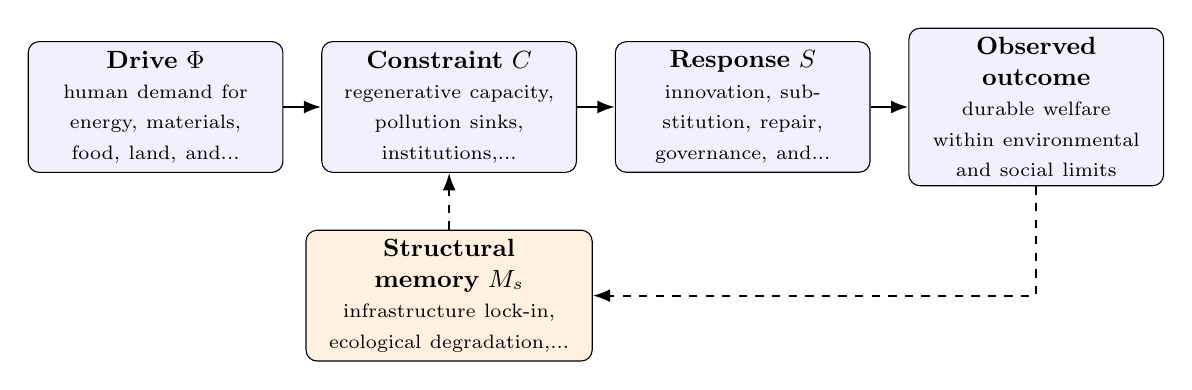
\begin{tikzpicture}[
    node distance=0.48cm,
    every node/.style={font=\small},
    box/.style={draw, rounded corners, align=center, minimum height=1.45cm, text width=3.0cm, fill=blue!6},
    memory/.style={draw, rounded corners, align=center, minimum height=1.25cm, text width=3.4cm, fill=orange!12},
    flow/.style={-{Latex[length=2.2mm]}, thick},
    feedback/.style={-{Latex[length=2.2mm]}, thick, dashed}
]
\node[box] (drive) {\textbf{Drive $\Phi$}\\\scriptsize human demand for energy, materials, food, land, and...};
\node[box, right=of drive] (constraint) {\textbf{Constraint $C$}\\\scriptsize regenerative capacity, pollution sinks, institutions,...};
\node[box, right=of constraint] (response) {\textbf{Response $S$}\\\scriptsize innovation, substitution, repair, governance, and...};
\node[box, right=of response] (outcome) {\textbf{Observed outcome}\\\scriptsize durable welfare within environmental and social limits};
\node[memory, below=0.72cm of constraint] (memory) {\textbf{Structural memory $M_s$}\\\scriptsize infrastructure lock-in, ecological degradation,...};
\draw[flow] (drive) -- (constraint);
\draw[flow] (constraint) -- (response);
\draw[flow] (response) -- (outcome);
\draw[feedback] (outcome.south) |- (memory.east);
\draw[feedback] (memory.north) -- (constraint.south);
\end{tikzpicture}
\caption{Paper A-10 observable CDFD/AFL architecture for Earth Sustainability. Solid arrows give the proposed forward chain; dashed arrows make history-dependent feedback explicit.}
\label{fig:a10-architecture}
\end{figure}

\subsection{Paper-Specific Causal Hypothesis}

For this paper, the hypothesized causal sequence is specific. A change in
human demand for energy, materials, food, land, and welfare arrives faster than innovation, substitution, repair, governance, and demand adjustment can compensate.
This raises or redistributes regenerative capacity, pollution sinks, institutions, and distribution. If the load persists,
the retained state encoded by infrastructure lock-in, ecological degradation, wealth, and institutional history changes the next response, so a later event of equal
magnitude can produce a different trajectory in durable welfare within environmental and social limits. The
scientific task is to estimate that sequence against the best ordinary model of
the domain, not merely to redescribe the outcome after it occurs.

\subsection{Cross-Scale Translation Without Mechanistic Erasure}

For the Earth systems family, the cross-domain translation compares coupled transport, finite environmental capacity, buffering, and retained landscape or ecosystem state. It cannot erase conservation laws, geometry, or scale; it must expose where those domain equations create comparable overload and recovery structures. \cite{Holling1973,Turing1952,BakTangWiesenfeld1987}
The required scale declaration for this paper is years to centuries; communities to the planet. At short
scales, the key question is whether the incoming drive is transmitted,
buffered, or diverted. At intermediate scales, response changes effective
capacity and network exposure. At long scales, retained structure can alter the
state space itself. A result is genuinely cross-scale only when the aggregation
rule is stated and the same conclusion is not an artifact of averaging.

\subsection{Evidence Ladder and Discriminating Tests}

\begin{table}[htbp]
\centering
\small
\caption{Evidence ladder for Paper A-10. Each rung can fail independently.}
\begin{tabularx}{\textwidth}{|p{0.17\textwidth}|X|X|}
\hline
\textbf{Test} & \textbf{Design} & \textbf{Discriminating result} \\
\hline
Proxy audit & Measure material-flow accounts, life-cycle inventories, ecological indicators, and welfare series and preregister how each record maps to $\Phi$, $C$, $S$, $M_s$, and $Y$. & The mapping fails if proxies are non-identifiable, circular, or change meaning across cases. \\
\hline
Load ramp & Apply or observe a demand increase combined with a capacity loss while estimating the dominant constraint and response time. & A threshold claim requires a reproducible nonlinear change and uncertainty bounds, not a visually chosen breakpoint. \\
\hline
Recovery and memory & Match present load across units with different histories, then compare recovery paths. & The memory claim requires history-dependent divergence after current conditions are controlled. \\
\hline
Model comparison & Compare the baseline domain model with and without the CDFD/AFL state variables using held-out data. & The paper's stated falsifier is: the framework cannot outperform established sustainability accounting or identify trade-offs. \\
\hline
\end{tabularx}
\end{table}

\subsection{Research Programme and Boundary Conditions}

The immediate research programme has four steps. First, construct a documented
dataset from material-flow accounts, life-cycle inventories, ecological indicators, and welfare series and retain raw units before normalization.
Second, fit a baseline domain model and report its calibration and out-of-sample
error. Third, add the smallest identifiable CDFD/AFL state extension and test
whether it improves prediction of durable welfare within environmental and social limits. Fourth, repeat the
analysis across the declared scale range and publish negative cases as part of
the cross-domain translation audit.

% END PART IV MAJOR CROSS-DOMAIN UPGRADE

\section{Conclusion}
Sustainability is not an ideological preference; it is a mathematical boundary condition. By applying CDFD, we establish the absolute thermodynamic limits of human expansion. Achieving a sustainable future requires abandoning the pursuit of infinite flux ($\Phi$) and instead mastering the topological elasticity ($S$) required to thrive within the unyielding constraints of our planetary surface.
\section*{Conflict of Interest} The author declares no conflict of interest.
\section*{Data Availability}
Part-specific runtime diagnostics are under each Part's \path{outputs/} directory.

Release-wide code: \path{Part_E_Synthesis/supplementary/}.

Generated summaries: \path{Part_E_Synthesis/outputs/}.

Figures: \path{Part_E_Synthesis/figures/}.


\section{Reference Layer}
\bibliographystyle{plain}
\bibliography{universal_afl_references}
\end{document}
